% Deepfake Detection — IITG Term Project Report (IEEEtran, template format)
\documentclass[conference]{IEEEtran}
\IEEEoverridecommandlockouts

\usepackage[utf8]{inputenc}
\usepackage[T1]{fontenc}
\usepackage{amsmath,amssymb}
\usepackage{graphicx}
\usepackage{booktabs}
\usepackage{cite}
\usepackage{url}
\usepackage{hyperref}
\usepackage{xcolor}
\usepackage{tikz}
\usetikzlibrary{arrows.meta,positioning}
\hypersetup{colorlinks=true,linkcolor=black,citecolor=black,urlcolor=blue,
  pdftitle={Deepfake Video Detection with Spatial-Temporal Networks},pdfauthor={Saket Kumar}}

% --- TEMPLATE FORMAT: Arabic numbering for sections, figures, tables ---
\renewcommand{\thesection}{\arabic{section}}
\renewcommand{\thesubsection}{\thesection.\arabic{subsection}}
\renewcommand{\thesubsubsection}{\thesubsection.\arabic{subsubsection}}
\renewcommand{\thefigure}{\arabic{figure}}
\renewcommand{\thetable}{\arabic{table}}
\makeatletter
\def\thesectiondis{\thesection.}
\def\thesubsectiondis{\thesection.\arabic{subsection}.}
\def\thesubsubsectiondis{\thesection.\arabic{subsection}.\arabic{subsubsection}.}
\renewenvironment{abstract}{%
  \par\addvspace{0.5\baselineskip}%
  \bgroup\centering\@IEEEabskeysecsize\textbf{ABSTRACT}\par\addvspace{0.5\baselineskip}\egroup%
  \quotation\@IEEEabskeysecsize%
}{\endquotation\par}
\renewenvironment{thebibliography}[1]{%
  \section{\refname}%
  \list{\@biblabel{\@arabic\c@enumiv}}%
       {\settowidth\labelwidth{\@biblabel{#1}}%
        \leftmargin\labelwidth
        \advance\leftmargin\labelsep
        \@openbib@code
        \usecounter{enumiv}%
        \let\p@enumiv\@empty
        \renewcommand\theenumiv{\@arabic\c@enumiv}}%
  \sloppy
  \clubpenalty4000
  \@clubpenalty \clubpenalty
  \widowpenalty4000%
  \sfcode`\.\@m}
 {\def\@noitemerr
   {\@latex@warning{Empty `thebibliography' environment}}%
  \endlist}
\makeatother

\begin{document}

\title{DEEPFAKE VIDEO DETECTION --- SPATIAL-TEMPORAL CNN/TRANSFORMER WITH CROSS-GENERATOR ARTIFACT ANALYSIS}

\author{\IEEEauthorblockN{Saket~Kumar~(Roll~Number:~23035010051)}\\[2mm]
\IEEEauthorblockA{Term Project Report}\\[1mm]
\IEEEauthorblockA{Trimester 9}\\[1mm]
\IEEEauthorblockA{B.Sc. (Honours) Data Science and Artificial Intelligence}\\[1mm]
\IEEEauthorblockA{Indian Institute of Technology Guwahati, India}\\[2mm]
\IEEEauthorblockA{Email: \texttt{k.saket@op.iitg.ac.in}}}

\maketitle

\begin{abstract}
Deepfake videos---face swaps, re-enactments, and attribute edits produced by generative models---are increasingly used for misinformation and impersonation, yet most detectors are evaluated only on the generators they were trained on. This report presents a deepfake video detection system whose objective is twofold: to classify manipulated videos reliably, and to study \emph{which manipulation artifacts generalize across generators}. A two-stage architecture was developed: an EfficientNet-B0 spatial detector scores individual face frames, and frame-level evidence is aggregated into a video-level verdict either by mean pooling or by a three-layer temporal transformer. The system was trained on FaceForensics++ (five manipulation generators) and evaluated with Celeb-DF v2 as a held-out cross-dataset test, under strictly video-level disjoint splits, a frame-count-controlled protocol, and CPU-only compute. The mean-pool spatial detector achieves a video-level AUC of 0.9553 (91.7\% accuracy) on the held-out test split and 0.9033 AUC across sources. Spectral (FFT) and Grad-CAM analyses identify high-frequency upsampling fingerprints as the strongest cue, while a cross-preprocessing study (AUC dropping to 0.6419) shows these artifacts are pipeline-dependent. A privacy-preserving browser demo runs the model entirely on-device via ONNX/WebAssembly.
\end{abstract}

\begin{IEEEkeywords}
Deepfake Detection, Digital Forensics, EfficientNet, Temporal Transformer, Cross-Generator Generalization, Spectral Analysis.
\end{IEEEkeywords}

\section{Introduction}
Generative face-manipulation models can now produce videos that are visually indistinguishable from genuine footage. Such ``deepfakes'' have been deployed in political disinformation, financial fraud, and non-consensual impersonation, making automatic detection a problem of practical and societal importance. A large body of forensic methods exists, but most detectors are trained and evaluated on a single manipulation dataset; their accuracy typically collapses when confronted with a generator they have not seen. The core difficulty is that a detector may learn \emph{dataset-specific} artifacts---compression, cropping pipelines, or generator fingerprints---rather than manipulation cues that transfer.

This project develops a deepfake video detection system and, beyond accuracy, asks a research question: \emph{which manipulation artifacts generalize across generators?} The system combines an EfficientNet-B0 spatial detector that scores individual face frames with a temporal transformer that aggregates frame embeddings into a video-level verdict. FFT spectral and Grad-CAM attention analyses characterize the cues the detector relies on, and a deliberately hard cross-preprocessing evaluation quantifies how those cues degrade when the face-crop pipeline differs from training.

All experiments use CPU-only hardware, and the model is deployed as a fully on-device browser demo. Section~2 defines the problem and objectives, Section~3 details the methodology, Section~4 presents results, Section~5 discusses them, and Sections~6--7 conclude and list reproducible artifacts.

\section{Problem Statement and Objectives}
\subsection{Problem Statement}
Given an input video, the task is binary video-level classification: decide whether the footage is genuine or has been manipulated by a face-synthesis method (face swap, re-enactment, attribute transfer, or entire-face generation). The scope is forensic screening of facial manipulation in compressed video; audio forensics and full-frame scene manipulation are out of scope. Three aspects make the problem hard: public dataset mirrors contain split leakage and frame-count shortcuts that silently inflate accuracy, so a trustworthy evaluation protocol must precede any model comparison; manipulation artifacts differ by generator family (swap-based methods modify only the face interior, autoencoder-based methods resynthesize it); and any deployed detector must run without uploading private footage.

\subsection{Objectives}
The specific objectives were: (1) to study existing deepfake detection approaches and datasets; (2) to design and implement a spatial-temporal detector---an EfficientNet-B0 frame scorer with temporal aggregation---trainable on CPU; (3) to construct leak-free, video-level disjoint train/val/test splits and a length-control protocol that removes the frame-count shortcut; (4) to evaluate video-level performance with AUC, average precision, and accuracy, including cross-dataset generalization to Celeb-DF v2; (5) to analyze which artifacts generalize using FFT spectral divergence and Grad-CAM attention; and (6) to deploy the detector as a zero-backend, on-device browser application.

\begin{figure*}[t]
\centering
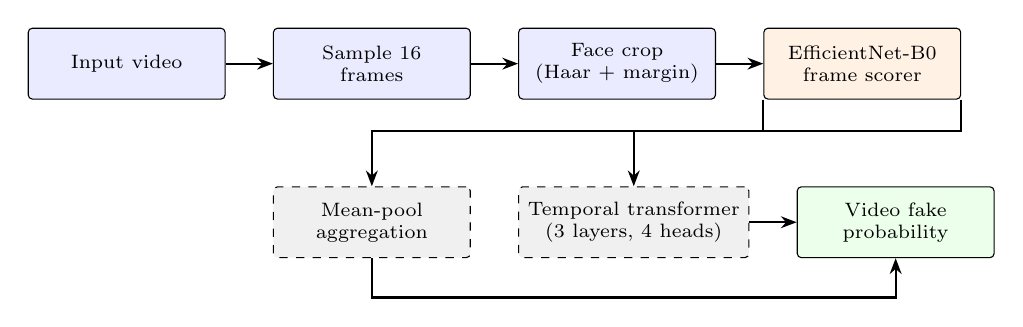
\begin{tikzpicture}[node distance=2mm and 6mm,
  box/.style={draw,rounded corners=1.5pt,minimum width=2.5cm,minimum height=0.9cm,
    align=center,font=\scriptsize},
  arr/.style={-{Stealth[length=2mm]},thick},
  obox/.style={draw,dashed,rounded corners=1.5pt,minimum width=2.5cm,minimum height=0.9cm,
    align=center,font=\scriptsize,fill=gray!12}]
  \node[box,fill=blue!8] (vid) {Input video};
  \node[box,fill=blue!8,right=6mm of vid] (frm) {Sample 16\\frames};
  \node[box,fill=blue!8,right=6mm of frm] (crop) {Face crop\\(Haar + margin)};
  \node[box,fill=orange!10,right=6mm of crop] (eff) {EfficientNet-B0\\frame scorer};
  \node[obox,below=11mm of frm] (pool) {Mean-pool\\aggregation};
  \node[obox,right=6mm of pool] (tt) {Temporal transformer\\(3 layers, 4 heads)};
  \node[box,fill=green!8,right=6mm of tt] (verd) {Video fake\\probability};
  \draw[arr] (vid) -- (frm);
  \draw[arr] (frm) -- (crop);
  \draw[arr] (crop) -- (eff);
  \draw[arr] (eff.south west) -- ++(0,-4mm) -| (pool.north);
  \draw[arr] (eff.south east) -- ++(0,-4mm) -| (tt.north);
  \draw[arr] (pool.south) -- ++(0,-5mm) -| (verd.south);
  \draw[arr] (tt) -- (verd);
\end{tikzpicture}
\caption{Overview of the detection pipeline. Sixteen evenly sampled frames are face-cropped and scored independently by EfficientNet-B0. Video-level evidence is aggregated either by mean pooling of frame scores (best result) or by a temporal transformer over frame embeddings; both paths yield a single fake probability for the whole video.}
\label{fig:pipeline}
\end{figure*}

\section{Methodology / Approach}
\subsection{Overall Workflow}
Figure~\ref{fig:pipeline} summarizes the pipeline. From each video, 16 frames are evenly sampled; a Haar-cascade face detector with a bounding-box margin extracts face crops. The spatial branch passes every crop through EfficientNet-B0 (ImageNet-initialized) to produce a per-frame fake probability. For video-level inference, frame scores are aggregated by mean pooling. As an alternative, frame embeddings (dimension 1280) are cached and consumed by a temporal transformer that learns to aggregate over the frame sequence.

\subsection{Technical Details}
\emph{Spatial detector.} EfficientNet-B0~\cite{tan2019efficientnet} was chosen for its accuracy-to-size ratio under CPU budgets. Training proceeds in two phases to keep compute tractable: first the classification head only (binary cross-entropy loss), then full fine-tuning on a class-balanced subset. Validation AUC improved from 0.7910 (head-only) to 0.8750 after fine-tuning and to 0.9100 after balanced fine-tuning.

\emph{Temporal aggregation.} Frame embeddings are projected to 256 dimensions, augmented with positional embeddings, and processed by a 3-layer, 4-head transformer~\cite{vaswani2017attention} with a CLS token and attention pooling, producing a video-level fake probability. Because clip lengths differ systematically between classes in the data mirror (Section~5), all temporal experiments use a length-control protocol: every clip is subsampled to exactly $T=2$ frames and shorter clips are dropped, so the model cannot exploit clip length as a feature.

\emph{Artifact analysis.} Two probes answer the generalization question. (1) \emph{Spectral fingerprints:} for each source, the radial power spectrum of fake frames is compared against real frames via an L1 divergence, decomposed into low/mid/high frequency bands; GAN-style decoders are known to leave periodic upsampling structure in the mid/high bands~\cite{durall2020fourier,wang2020cnngen}. (2) \emph{Spatial attention:} Grad-CAM~\cite{selvaraju2020gradcam} maps are reduced to a center-of-mass statistic (0 = image center) to test whether the detector attends to the manipulated face interior or to borders and compression.

\subsection{Project Architecture}
The implementation is a single Python package (\texttt{deepfake\_detection}) with YAML-configured stages: \texttt{prepare\_data.py} builds leak-free video-disjoint splits; \texttt{models/spatial.py} and \texttt{models/temporal.py} define the two networks; \texttt{train\_spatial.py} and \texttt{train\_temporal.py} run training and AUC evaluation; \texttt{analyze\_generalization.py} and \texttt{analyze\_artifacts.py} produce the per-generator study and FFT/Grad-CAM reports; and \texttt{export\_onnx.py} exports an fp16 ONNX model consumed by the static browser app, which pairs MediaPipe BlazeFace~\cite{lugaresi2019mediapipe} with ONNX Runtime Web (WASM) for fully client-side inference. Unit tests cover parsing, models, metrics, and preprocessing.

\section{Experiments and Results}
\subsection{Experimental Setup}
\emph{Data.} The primary corpus is pre-extracted face frames from FaceForensics++ (C23)~\cite{rossler2019ff} covering five generators (Deepfakes, Face2Face, FaceSwap, NeuralTextures, FaceShifter), with Celeb-DF v2~\cite{li2020celebdf} as a held-out, out-of-distribution test source; face crops use a Haar cascade~\cite{viola2004robust} with margin. \emph{Protocol.} Splits are video-level disjoint (1{,}044 leaked training rows dropped); all models train on CPU. \emph{Metrics.} Video-level AUC (threshold-independent), average precision (AP), and accuracy; the held-out test set comprises 1{,}289 videos.

\subsection{Results}
\emph{Video-level benchmark.} Table~\ref{tab:benchmark} reports the main results under length control ($T=2$); mean-pooling of spatial frame scores is the strongest configuration.

\begin{table}[htbp]
\caption{Video-level benchmark on the held-out test split ($n=1289$, length-controlled $T=2$). Best result in bold.}
\label{tab:benchmark}
\centering
\renewcommand{\arraystretch}{1.15}
\begin{tabular}{@{}lccc@{}}
\toprule
Model / aggregation & AUC & AP & Acc.\\
\midrule
Spatial, mean-pool & \textbf{0.9553} & \textbf{0.9838} & \textbf{0.9170}\\
Spatial, max-pool & 0.9336 & 0.9764 & 0.8960\\
Spatial, top-$k$ & 0.9336 & 0.9764 & 0.8960\\
Spatial + temporal transformer & 0.9456 & 0.9768 & 0.8813\\
\bottomrule
\end{tabular}
\end{table}

\emph{Cross-source generalization.} With one model trained on the FaceForensics++ mix, Table~\ref{tab:crosssource} shows performance per held-out source, including 0.9220 AUC on the out-of-distribution Celeb-DF v2 family.

\begin{table}[htbp]
\caption{Cross-source generalization of a single model on held-out test videos.}
\label{tab:crosssource}
\centering
\renewcommand{\arraystretch}{1.15}
\begin{tabular}{@{}lcc@{}}
\toprule
Source & Test AUC & $n$\\
\midrule
Celeb-DF v2 (OOD family) & 0.9220 & 3{,}000\\
FaceForensics++ & 0.8928 & 1{,}916\\
Overall & 0.9033 & --\\
\bottomrule
\end{tabular}
\end{table}

\emph{Cross-preprocessing generalization.} When test frames come from a \emph{different} face-crop pipeline than training, per-generator results (Table~\ref{tab:crossgen}) degrade sharply: autoencoder-based Deepfakes remain detectable (0.8011 AUC) while swap-based forgeries fall to 0.56--0.63 AUC.

\begin{table}[htbp]
\caption{Per-generator AUC under cross-preprocessing evaluation (different face-crop pipeline than training).}
\label{tab:crossgen}
\centering
\renewcommand{\arraystretch}{1.15}
\begin{tabular}{@{}lcc@{}}
\toprule
Generator & Test AUC & $n$\\
\midrule
Deepfakes & 0.8011 & 1{,}394\\
Face2Face & 0.6291 & 1{,}399\\
NeuralTextures & 0.6220 & 1{,}399\\
FaceShifter & 0.5955 & 1{,}398\\
FaceSwap & 0.5629 & 1{,}398\\
\midrule
Overall & 0.6419 & 6{,}988\\
\bottomrule
\end{tabular}
\end{table}

\emph{Artifact analysis.} FF++ fakes deviate from real frames 2.3$\times$ more in the radial power spectrum than Celeb-DF fakes (L1 0.054 vs.\ 0.024), driven by the high-frequency band (0.025 vs.\ 0.009)---the classic decoder upsampling fingerprint. Grad-CAM center-of-mass statistics show fakes pull attention into the face interior (0.32 Celeb-DF, 0.22 FF++) whereas real frames scatter (0.09), confirming the detector keys on manipulated facial content rather than borders or compression.

\section{Discussion}
Two data-integrity problems were found and fixed, and both materially affect reported accuracy. The Kaggle mirror's provided splits leaked 124 validation and 78 test videos into training; without rebuilding video-disjoint splits, every metric in Table~\ref{tab:benchmark} would be optimistically biased. Additionally, real clips in the mirror contain 12 frames while fakes contain only 2--3, so a temporal model can achieve a perfect AUC merely by \emph{counting frames}; the length-control protocol ($T=2$) removes this shortcut.

The mean-pool aggregator outperforming the temporal transformer (0.9553 vs.\ 0.9456 AUC) is interpretable: under length control each clip contributes very few frames, leaving the transformer little sequential structure, while averaging is a robust, variance-reducing estimator of frame-level evidence. The cross-preprocessing study is the main negative finding: artifacts generalize well \emph{within} a preprocessing pipeline (AUC 0.90--0.96) but degrade sharply \emph{across} pipelines (0.56--0.80); swap-based forgeries leave the weakest cue because they modify only the face interior, whereas autoencoder-based methods resynthesize the whole crop and leave stronger decoder fingerprints. On the deployment side, int8 quantization was rejected (it collapses EfficientNet's squeeze-and-excitation blocks, dropping frame AUC from 0.97 to 0.55); fp16 export halves model size with no measurable loss. The principal limitation is thus pipeline dependence: a production system would need multi-pipeline training data or preprocessing-invariant features, and detection scores should be read as forensic evidence cues, not legal proof.

\section{Conclusion and Future Work}
This project delivered a CPU-trained deepfake detector achieving 0.9553 video-level AUC on a leak-free, length-controlled test split (0.9033 across sources, including an out-of-distribution generator family), an artifact study identifying high-frequency spectral fingerprints as the strongest but pipeline-dependent cue, and a fully on-device browser deployment. The key insight is that within-pipeline benchmark accuracy overstates real-world robustness. Future work includes joint multi-pipeline, multi-generator training, preprocessing-invariant representations, and adversarial robustness testing.

\section{Artifacts and Demonstrations}
All artifacts are publicly accessible. \emph{Code repository:} \url{https://github.com/saketkumar-18/deepfake-detection} (full source, configs, unit tests, training logs, and analysis scripts). \emph{Live demo:} \url{https://deepfake-detector-amber.vercel.app} --- a zero-backend browser app running the detector fully on-device via fp16 ONNX in WebAssembly. \emph{Video demonstration:} the accompanying video submission is on YouTube.

\newpage
\begin{thebibliography}{99}
\bibitem{rossler2019ff} A.~R\"ossler, D.~Cozzolino, L.~Verdoliva, C.~Riess, J.~Thies, and M.~Nie\ss{}ner, ``FaceForensics++: Learning to detect manipulated facial images,'' in \emph{Proc. IEEE/CVF Int. Conf. Computer Vision (ICCV)}, 2019, pp. 1--11.
\bibitem{li2020celebdf} Y.~Li, X.~Yang, P.~Sun, H.~Qi, and S.~Lyu, ``Celeb-DF: A large-scale challenging dataset for deepfake forensics,'' in \emph{Proc. IEEE/CVF Conf. Computer Vision and Pattern Recognition (CVPR)}, 2020, pp. 3207--3216.
\bibitem{tan2019efficientnet} M.~Tan and Q.~V.~Le, ``EfficientNet: Rethinking model scaling for convolutional neural networks,'' in \emph{Proc. Int. Conf. Machine Learning (ICML)}, 2019, pp. 6105--6114.
\bibitem{vaswani2017attention} A.~Vaswani \emph{et al.}, ``Attention is all you need,'' in \emph{Advances in Neural Information Processing Systems (NeurIPS)}, vol.~30, 2017, pp. 5998--6008.
\bibitem{selvaraju2020gradcam} R.~R.~Selvaraju, M.~Cogswell, A.~Das, R.~Vedantam, D.~Parikh, and D.~Batra, ``Grad-CAM: Visual explanations from deep networks via gradient-based localization,'' \emph{Int. J. Computer Vision}, vol.~128, no.~2, pp. 336--359, 2020.
\bibitem{durall2020fourier} R.~Durall, M.~Keuper, and J.~Laaksonen, ``Unmasking deepfakes with simple Fourier analysis,'' in \emph{Proc. IEEE/CVF Conf. Computer Vision and Pattern Recognition Workshops (CVPRW)}, 2020, pp. 2892--2897.
\bibitem{wang2020cnngen} S.-Y.~Wang, O.~Wang, R.~Zhang, A.~Owens, and A.~A.~Efros, ``CNN-generated images are surprisingly easy to spot\ldots for now,'' in \emph{Proc. IEEE/CVF Conf. Computer Vision and Pattern Recognition (CVPR)}, 2020, pp. 8695--8704.
\bibitem{viola2004robust} P.~Viola and M.~J.~Jones, ``Robust real-time face detection,'' \emph{Int. J. Computer Vision}, vol.~57, no.~2, pp. 137--154, 2004.
\bibitem{lugaresi2019mediapipe} C.~Lugaresi \emph{et al.}, ``MediaPipe: A framework for building perception pipelines,'' \emph{arXiv preprint arXiv:1906.08172}, 2019.
\bibitem{onnxruntime2024} Microsoft, ``ONNX Runtime: Cross-platform inference and training accelerator,'' 2024. [Online]. Available: \url{https://onnxruntime.ai/}
\bibitem{kaggleframes2024} wish096, ``FF and CelebDF frame dataset,'' Kaggle Datasets, 2024. [Online]. Available: \url{https://www.kaggle.com/datasets/wish096/ff-andcelebdf-frame-dataset-by-wish}
\end{thebibliography}

\end{document}
